\chapter{Sistemi MIMO nel dominio di Laplace}

\section{Rappresentazione di un sistema MIMO nel dominio di Laplace}


Consideriamo il seguente sistema LTI 
a più ingressi e più uscite (MIMO) descritto dalle seguenti equazioni:
\begin{equation}
    \begin{cases}
        \dot{x}(t) = Ax(t) + Bu(t) \\
        y(t) = Cx(t) + Du(t)
    \end{cases}
\end{equation}
Il sistema è MIMO dunque \( u \in \mathbb{R}^{m \times 1}\),
\(y \in \mathbb{R}^{p \times 1}\),
\(B \in \mathbb{R}^{n \times m}\),
\(C \in \mathbb{R}^{p \times n}\)
e \(D \in \mathbb{R}^{p \times m}\).
Il sistema può essere rappresentato nel dominio di Laplace come:
\begin{equation}
    Y(s) = G(s)U(s) 
\end{equation}
Con \( G(s) \in \mathbb{R}^{p \times m} \) matrice di trasferimento del sistema
definita come:
\begin{equation}
    G(s) = C(sI - A)^{-1}B + D
\end{equation}
La matrice \(G(s)\) è composta da \(p \times m\) funzioni di trasferimento
singole \(G_{ij}(s)\):
\[G(s) = \begin{pmatrix}
    G_{11}(s) & \ldots & G_{1m}(s) \\
    \vdots & \vdots & \vdots \\
    G_{p1}(s) & \ldots & G_{pm}(s)
\end{pmatrix}\]
dove ogni elemento \(G_{ij}(s)\) è una funzione polinomiale 
fratta che rappresenta la funzione di trasferimento
tra l'ingresso \(u_j\) e l'uscita \(y_i\).

\section{Sistema con retroazione dell'uscita MIMO}
Consideriamo lo schema di controllo a retroazione
dell'uscita per un sistema MIMO mostrato in Figura \ref{fig:sistema_mimo_retroazione}.
Andiamo ora a ricavarci le funzioni di trasferimento del sistema considerando come 
uscite i due vettori \(Y(s) \in \mathbb{R}^{p}\) e
\(U(s) \in \mathbb{R}^{m}\), e come ingresso i quattro vettori 
\(R(s), D_u(s), D_y(s), N(s)\). Per prima cosa definiamo la funzione 
d'anello aperto \(L(s)\) è definita come:
\[L(s) \coloneq G(s)K(s)\]
Notiamo che \(K(s)G(s)\) a priori è diverso poichè stiamo parlando di matrici
ed il prodotto tra matrici non è commutativo. Definiamo anche la 
\textbf{funzione di sensitività}:
\[S(s) \coloneq \left(I + L(s)\right)^{-1}\]
e la \textbf{funzione di sensitività complementare}:
\[T(s) \coloneq\left(I + L(s)\right)^{-1} L(s)  \]
Andiamo a trovarci le funzioni di trasferimento tra le uscite e gli ingressi,
nello specifico saranno otto funzioni di trasferimento:
\begin{enumerate}
  \item Funzione di trasferimento tra \(R(s)\) a \(Y(s)\), che vale:
  \[K_{YR} = T(s) = \left(I + L(s)\right)^{-1} L(s)  \]
  \item Funzione di trasferimento tra \(Y(s)\) e \(D_u(s)\), che vale:
  \[ K_{YD_{u}}(s) \coloneq \left(I + L(s)\right)^{-1}G(s) = S(s) G(s) \]
  \item Funzione di trasferimento tra \(Y(s)\) e \(D_y(s)\), che vale:
  \[ K_{Y D_{y}}(s) \coloneq \left(I + L(s)\right)^{-1} = S(s) \]
  \item Funzione di trasferimento tra  \(Y(s)\) e \(N(s)\) , che vale:
  \[ K_{YN}(s) \coloneq -\left(I + L(s)\right)^{-1}L(s) = -T(s) \]
  \item Funzione di trasferimento tra  \(U(s)\) e \(R(s)\), che vale:
  \[ K_{UR}(s) \left(I + K(s) G(s)\right)^{-1} K(s)\]
  \item Funzione di trasferimento tra \(U(s)\) e \(D_u(s)\), che vale:
  \[ \left(I + K(s) G(s)\right)^{-1} \]
  \item Funzione di trasferimento tra \(U(s)\) e \(D_y(s)\), che vale:
  \[ -\left(I + K(s) G(s)\right)^{-1} K(s) \]
  \item Funzione di trasferimento tra \(U(s)\) e \(N(s)\), che vale:
  \[ -\left(I + K(s) G(s)\right)^{-1} K(s)\]
\end{enumerate}

Dunque il legame tra \(Y(s)\) e \(U(s)\) con gli ingressi
\(R(s), D_u(s), D_y(s), N(s)\) è dato da:
\[Y(s) = S(s)G(s) D_{u}(s) + S(s) D_{y}(s) - T(s) N(s) + T(s) R(s) \]
\[U(s) = \left(I + L_{u}\right) ^{-1}K(s) (R(s) - D_{y}(s) - N(s))  +
\left(I+ L_{u}(s)\right)^{-1} D_{u}(s)\]
\begin{figure}[tbp]
    \centering
    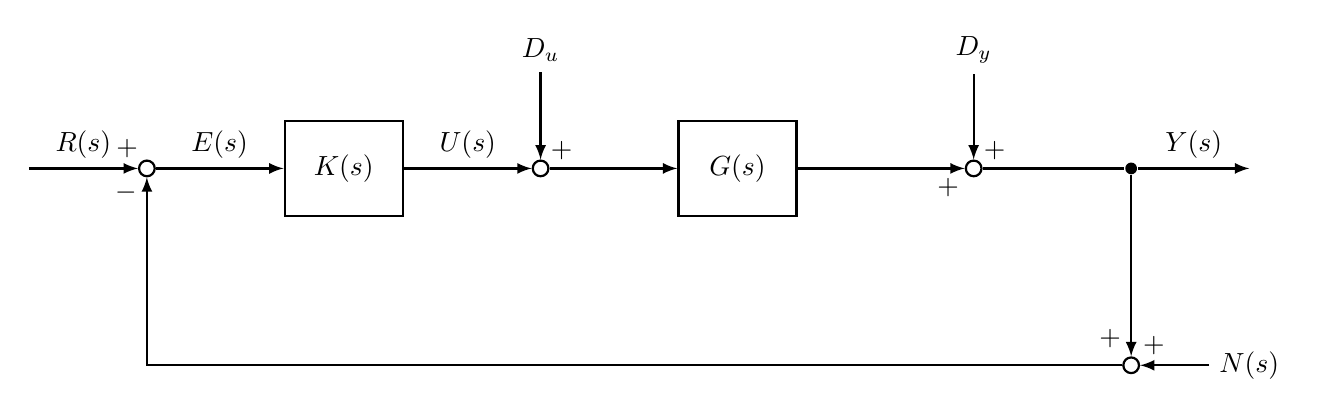
\begin{tikzpicture}[auto, node distance=2cm, >=latex, thick]
        % Stili
        \tikzstyle{block} = [draw, rectangle, minimum height=1.2cm, minimum width=1.5cm, align=center]
        \tikzstyle{sum} = [draw, circle, inner sep=2pt]
        \tikzstyle{coord} = [coordinate]
        \tikzstyle{dot} = [fill=black, circle, inner sep=1.5pt]

        % --- Catena Diretta (Forward Path) ---
        \node [coord] (input) {};
        
        % Sommatore Errore
        \node [sum, right of=input, node distance=1.5cm] (sum1) {};
        
        % Controllore K(s)
        \node [block, right of=sum1, node distance=2.5cm] (controller) {$K(s)$};
        
        % Sommatore Disturbo su U
        \node [sum, right of=controller, node distance=2.5cm] (sum_u) {};
        
        % Processo G(s)
        \node [block, right of=sum_u, node distance=2.5cm] (plant) {$G(s)$};
        
        % Sommatore Disturbo su Y
        \node [sum, right of=plant, node distance=3.0cm] (sum_y) {};
        
        % Punto di prelievo (Measure Point) - Un po' più avanti del sommatore
        \node [dot, right of=sum_y, node distance=2cm] (measure_point) {};
        
        % Uscita finale
        \node [coord, right of=measure_point, node distance=1.5cm] (output) {};

        % --- Nodi per i Disturbi ---
        \node [above of=sum_u, node distance=1.5cm] (du) {$D_u$};
        \node [above of=sum_y, node distance=1.5cm] (dy) {$D_y$};

        % --- Retroazione ---
        % Sommatore per il Rumore N(s) - Allineato verticalmente sotto il punto di prelievo
        \node [sum, below of=measure_point, node distance=2.5cm] (sum_noise) {};
        % Rumore N(s)
        \node [right of=sum_noise, node distance=1.5cm] (noise) {$N(s)$};

        % --- Collegamenti ---
        
        % Ingresso -> Sommatore 1
        \draw [->] (input) -- node {$R(s)$} node[pos=0.9, above] {$+$} (sum1);
        
        % Sommatore 1 -> K(s)
        \draw [->] (sum1) -- node {$E(s)$} (controller);
        
        % K(s) -> Sommatore Du
        \draw [->] (controller) -- node {$U(s)$} (sum_u);
        
        % Disturbo Du -> Sommatore Du
        \draw [->] (du) -- node[pos=0.9, right] {$+$} (sum_u);
        
        % Sommatore Du -> G(s)
        \draw [->] (sum_u) -- (plant);
        
        % G(s) -> Sommatore Dy
        \draw [->] (plant) -- node[pos=0.9, below] {$+$} (sum_y);
        
        % Disturbo Dy -> Sommatore Dy
        \draw [->] (dy) -- node[pos=0.9, right] {$+$} (sum_y);
        
        % Sommatore Dy -> Punto di prelievo -> Uscita
        \draw [->] (sum_y) -- (measure_point) -- node [name=y_out] {$Y(s)$} (output);

        % --- Collegamenti Retroazione ---
        % Scende dal punto di prelievo (measure_point) verso il sommatore del rumore
        \draw [->] (measure_point) -- (sum_noise) node[pos=0.9, left]{ $+$};
        
        % Rumore -> Sommatore Rumore
        \draw [->] (noise) -- (sum_noise) node[pos=0.8, above] {$+$};
        
        % Ritorno al primo sommatore
        \draw [->] (sum_noise) -| (sum1) node[pos=0.96, left] {$-$};

    \end{tikzpicture}
    \caption{Schema a blocchi di un sistema MIMO con retroazione dell'uscita.}
    \label{fig:sistema_mimo_retroazione}
\end{figure}




\section{Guadagno}
Definiamo gli spazi \(L^{p}\)
come gli spazi delle funzioni \(p\)-sommabili,
cioè in cui esiste la norma \(p\)-esima finita:
\[L^{p}(\mathbb{R^{n}}) = 
\left\{f : \mathbb{R} \to \mathbb{R}^{n} : 
\int_{-\infty}^{+\infty} \left|\left|f(\tau)
\right|\right|^{p}_{p} \, d\tau < \infty \right\}\]
Dove essendo \(f\) una funzione vettoriale a variabile reale
la norma \(p\)-esima è definita come:
\[\left|\left|f(\tau)\right|\right|_{p} =
\left( \sum_{i=1}^{n} |f_{i}(\tau)|^{p} \right)^{\frac{1}{p}}\]
Dove con \(f_{i}(\tau)\) si intende la \(i\)-esima componente del vettore
\(f(\tau)\) (che è un vettore di \(n\) componenti in cui ognuna è una funzione 
di \(\tau\))
\section{Poli e zeri per sistemi MIMO }
Ora ci poniamo il problema di definire poli e zeri per sistemi MIMO.
Per i sistemi SISO i poli sono definiti come gli zeri del denominatore della 
funzione di trasferimento, mentre gli zeri sono definiti come gli zeri del numeratore
della funzione di trasferimento. Il problema è che per i sistemi MIMO
ho una matrice di trasferimento \(G(s)\) composta da \(pm\) funzioni 
di trasferimento singole \(G_{ij}(s)\), quindi bisogna dare una nuova 
definizione di poli e zeri per sistemi MIMO.
Per prima cosa diamo la definizione di polo per sistemi MIMO.

\begin{definizione}
    Un polo di un sistema MIMO è un valore di \(s\) tale che la matrice \(G(s)\)
    diventa singolare, cioè il suo determinante è nullo, dunque per quel valore di \(s\)
    la matrice \(G(s)\) non è invertibile.
\end{definizione}


\begin{definizione}
    Si definisce rango nominale di una matrice di polinomi 
    \(G(s)\), il rango della matrice che si ha per tutti i valori di 
    \(s\) eccetto un numero finito di valori.
\end{definizione}


\begin{definizione}
    Uno zero di un sistema MIMO è un valore di \(s\) tale 
    che la matrice \(G(s)\)
    perde rango, cioè il rango della matrice \(G(s)\) 
    diminuisce rispetto al suo rango nominale (quello che ha per 
    tutti gli altri valori di \(s\)).
\end{definizione}

